% !TeX root = ../thuthesis-example.tex

\chapter{引言}
\section{研究背景\label{sec:chap1-sec1}}
“物联网”这一术语通常指的是将网络的连接性和计算能力拓展到通常不被视为计算机的物体、传感器和日常物品,使这些设备能够在最小的人工干预下生成、交换和消费数据。物联网这一词汇最早由英国人 Kevin Ashton 在 1999 年用于描述一个系统,在该系统中,物理世界中的对象通过传感器连接到互联网\cite{li2015internet}。一些预测认为,到 2025 年,全球参与物联网的设备数可能达到 1000 亿台,对经济的影响超过 11 万亿美元\cite{rose2015internet}。

在 2013 年德国汉诺威工业展览会上,“工业 4.0”理念首度面世\cite{ghobakhloo2020industry},其中提及的工业物联网(Industrial Internet of Things, IIoT)在全球范围内引起了广泛关注。IIoT 关注将所有的工业资产,包括及其和控制系统,与信息系统和业务流程连接起来,从中收集的大量数据可以为工业生产、管理、解决方案设计提供重要的参考作用\cite{sisinni2018industrial}。工业物联网会产生大量工业数据,其类型包括时间序列、图片、视频、文档等,在某些场景下一年内甚至会产生 $4\times 10^{12}$ GB 数据\cite{ge2012riseofindustrial}。在这些数据中,时间序列数据主要由机器设备上的传感器采集产生,由于采集频率高、传感器数量多,成为了工业大数据的主体\cite{di2019industrial}。

工业物联网场景下传感器数量可能很多,写入数据的速率也很高。例如,一架波音 787 客机在一次飞行中就可以产生超过 512 GB 的时序数据\cite{ronkainen2015designing};上海地铁目前有 136 列地铁的传感器数据开始被收集和监控,一年产生的数据量超过 254 TB;长安汽车集团生产的每一辆汽车上均有数千个传感器,其车联网应用一共管理了近 12 亿条时间序列,每年产生的数据量超过 13,000 TB。

海量的时序数据对数据的写入、存储和查询都提出了挑战。传统的关系型数据库通常使用 B+ 树作为底层的存储数据结构,其在处理点写入、点查询等负载时具有较好的性能,但是在面对工业物联网场景下时序数据的高速率写入和聚合查询负载时性能较差,无法满足需求\cite{jensen2017time}。因此,一种专门为存储时序数据而设计的数据库应运而生,它们被称为时序数据库(Time Series Database,TSDB)。如图 \ref{fig:db-engine} 所示,在国际权威数据库流行度排行机构 DB-Engines 的调查结果中,时序数据库在过去十年内的流行度持续上升,目前其流行度仅次于图数据库,位居榜单中的第二名。

\begin{figure}
  \centering
  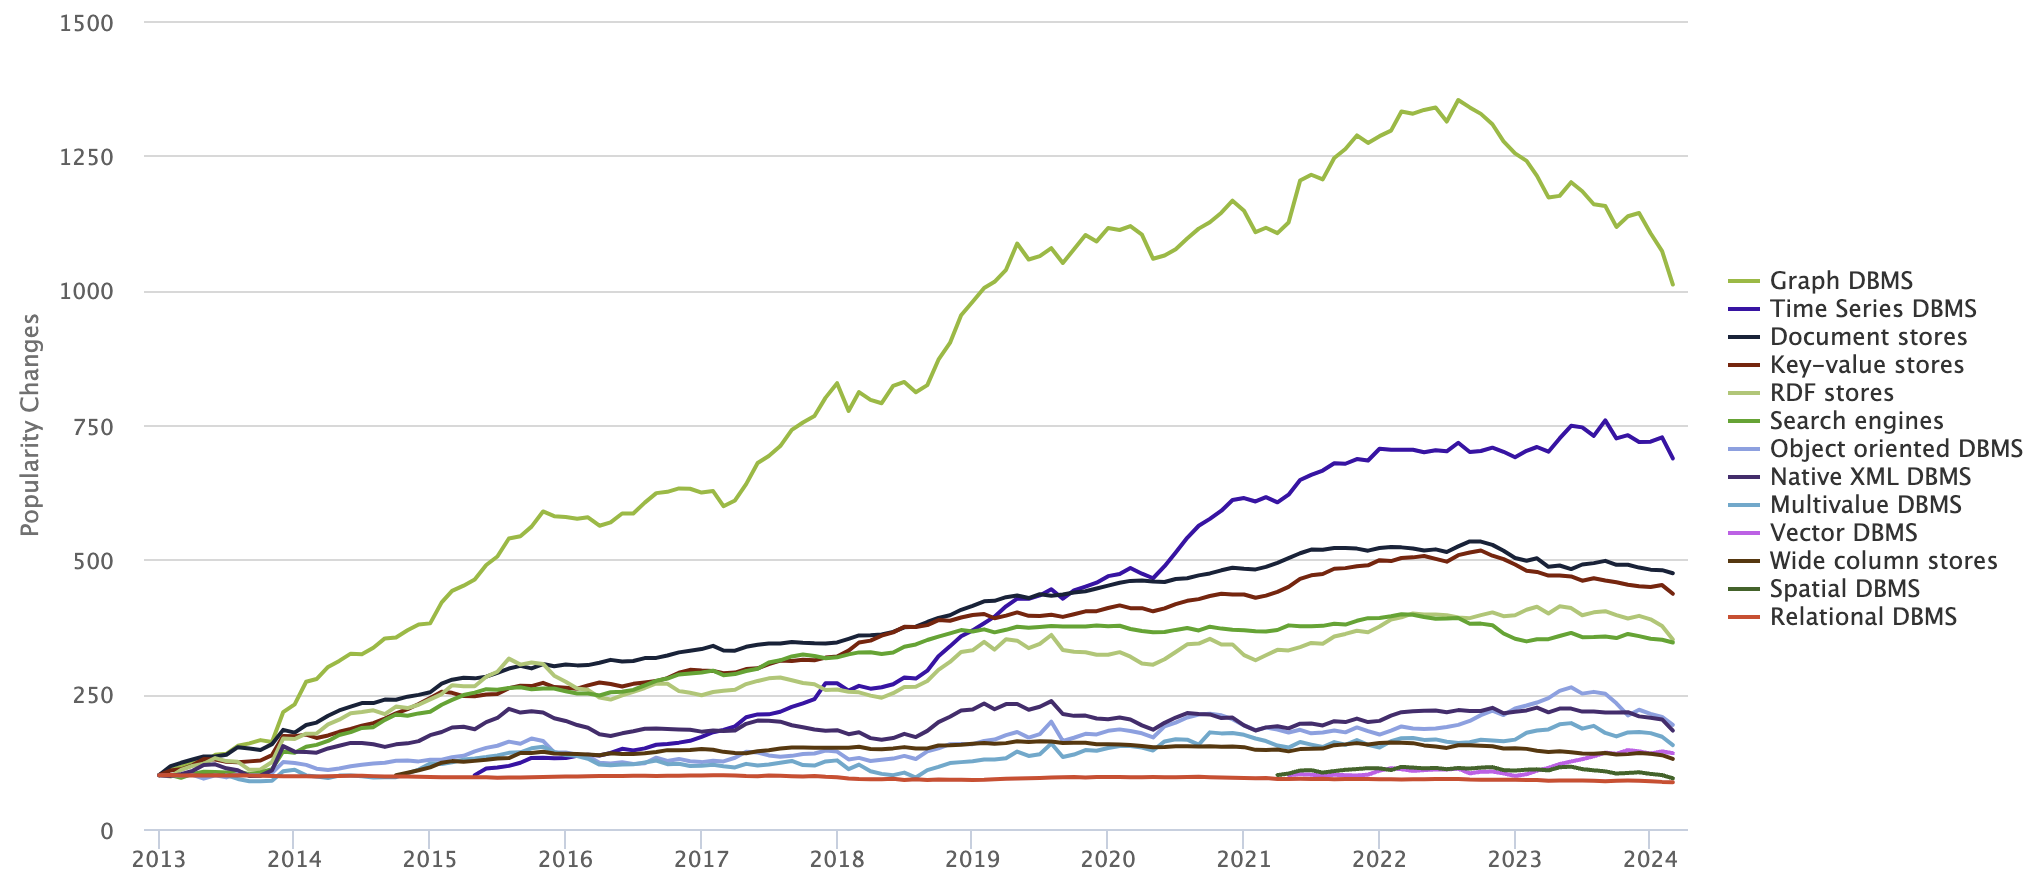
\includegraphics[width=\linewidth]{db-engines-ranking.png}
  \caption{DB-Engine 数据库类型流行度排名}
  \label{fig:db-engine}
\end{figure}

Apache IoTDB 是 Apache 基金会下一款开源的时序数据库,其具有为时间序列数据所优化的存储引擎、查询引擎以及分布式框架,可以满足工业物联网领域对海量时间序列数据高速写入、存储、快速读取以及复杂查询的需求\cite{wang2023apache}。

针对工业物联网场景下大量时序数据高速写入的需求,Apache IoTDB 主要提供了三种类型的数据写入接口:SQL 写入、原生列式写入接口、原生行式写入接口。在写入性能上,原生列式写入接口的性能最优,原生行式写入接口次之,SQL 写入性能最差;在写入的灵活性上,SQL 写入的灵活性最高,原生行式写入接口的灵活性次之,原生列式写入接口的灵活性最差。在大部分用户的使用场景中,SQL 式写入性能难以满足要求,原生列式写入接口则灵活性不足,使用原生行式写入接口可以兼具灵活性和良好的性能。但是,随着时序数据体量越来越大,原生行式接口写入较列式写入性能较差的问题显得越来越重要。例如,长安汽车车联网项目的一期工程有 12 亿条时间序列,采样周期为 30 秒,而二期工程不仅有 80 亿条时间序列,采样周期也减小到了 10 秒。如果原生行式写入接口的性能不变,粗略估计二期工程的服务器硬件成本约为一期的 20 倍。如果可以重新设计和实现一套高性能的行式写入机制,在负载相同的情况下就可以帮助用户降低机器的硬件成本,在负载越大的场景降成本的效果就越明显。设计和实现一套高性能的行式写入机制需要对客户端、网络传输、存储引擎等组件进行精心的设计和细致的优化。因此,提高 IoTDB 行式写入的性能具有一定的挑战性以及重要的实际意义和应用价值。
\section{Apache IoTDB 现有行式写入接口分析}
\subsection{Apache IoTDB 行式写入接口定义}
在 Apache IoTDB 中,时间序列采用树形的元数据结构进行描述。例如,某条时间序列可以被描述为 root.sg.d.s1,该字符串由多个“.”分隔开,“.”之间的字符则为元数据树中的一个节点。一条时间序列都倒数第二个节点被称为一个设备(Device),例如在前面的例子中 root.sg.d 就是一个设备。如果两个或多个时间序列都设备相同,那么则称这些时间序列是同一个设备下的序列。在大部分用户建模的场景中,设备通常对应了现实中的一个实体,例如一台机器或者一辆汽车,而设备下的每条序列则对应实体上部署的传感器。

IoTDB 提供的原生行式写入接口为 insertRecord 和 insertRecords,前者一次发送一行记录,而后者一次发送多行记录。为了减少由于网络传输带来的开销,大部分用户选择使用后者进行写入,本文所关注和研究的对象也主要是后者,即一次发送多行记录的写入形式。以 IoTDB 的 Java 客户端为例,insertRecord 和 insertRecords 接口的定义为:
\begin{lstlisting}[language=java,frame = trBL , firstnumber = last , escapeinside={(*@}{@*)}]
  void insertRecord(
      String deviceId,
      long time,
      List<String> measurements,
      List<TSDataType> types,
      List<Object> values
      )

  void insertRecords(
      List<String> deviceIds, 
      List<Long> times, 
      List<List<String>> measurementsList, 
      List<List<TSDataType>> typesList, 
      List<List<Object>> valuesList
      )
\end{lstlisting}
insertRecord 一次发送一行记录,这里的一行记录指的是这些数据属于一个设备下的时间序列,并且这些数据的时间戳都是相同的。表 \ref{tabular:insert-record-params} 详细介绍了该接口每个参数的含义。
\begin{table}
  \centering
  \caption{insertRecord 参数说明}
  \begin{tabular}{lll}
    \toprule
    参数名 &  类型 & 描述 \\
    \midrule
    deviceId & String & 数据所属的设备 ID \\
    time & long & 数据的时间戳 \\
    measurements & List<String> & 每个数据点所属的时间序列 ID 组成的列表 \\
    types & List<TSDataType> & 每个数据点所对应的数据类型 \\
    values & List<Object> & 每个数据点的数据 \\
    \bottomrule
  \end{tabular}
  \label{tabular:insert-record-params}
\end{table}

insertRecords 接口实际上是把多行记录一起从客户端发送到服务器,从接口的定义上看,每个与 insertRecord 接口对应的参数都变成了对应的列表,列表中的一个元素就描述了对应记录的相关信息,例如 deviceIds 中的每个元素就是每行记录对应的设备 ID。表\ref{tabular:insert-records-params} 中描述了 insertRecords 每个参数的含义。

\begin{table}
  \centering
  \caption{insertRecords 参数说明}
  \begin{tabular}{lll}
    \toprule
    参数名 &  类型 & 描述 \\
    \midrule
    deviceIds & List<String> & 每行记录所属的设备 ID 组成的列表 \\
     times & List<Long> & 每行记录的时间戳组成的列表 \\
    measurementsList & List<List<String> > & 每行记录的序列 ID 列表组成的列表 \\
    typesList & List<List<TSDataType> > & 每行记录数据类型列表组成的列表 \\
    valuesList & List<List<Object> > & 每行记录值列表组成的列表 \\
    \bottomrule
  \end{tabular}
  \label{tabular:insert-records-params}
\end{table}

综上,IoTDB 原生行式写入接口可以一次写入若干行记录,每条记录包含一个设备在一个时间戳下一条或若干条时间序列的数值。
\subsection{Apache IoTDB 现有行式写入机制实现}
\subsection{Apache IoTDB 现有行式写入机制不足}

\section{研究内容}
结合 \ref{sec:chap1-sec1} 和 \ref{sec:chap1-sec2} 节的分析,本文有以下发现:
\begin{enumerate}
  \item 在 Apache IoTDB 提供的三种写入接口中,原生行式写入接口具有较好的性能和灵活度,在大部分用户的场景下都适合适用。但是由于行式写入接口与列式写入接口具有一定的性能差距,在时间序列量较大的情况下无法满足用户的性能需求,也没有将服务器的资源高效利用。
  \item 
\end{enumerate}
\section{研究贡献}
\section{本文的组织结构}